%% supplementary/supplementary.tex — Steps D1, D2, H3
\documentclass[12pt]{article}
\usepackage{amsmath,amssymb,booktabs,graphicx,subcaption,float,hyperref}
\usepackage[margin=2.5cm]{geometry}

\renewcommand{\thefigure}{S\arabic{figure}}
\renewcommand{\thetable}{S\arabic{table}}
\renewcommand{\thesection}{S\arabic{section}}
\setcounter{figure}{0}
\setcounter{table}{0}

\title{Supplementary Material:\\
NLP-Augmented Multimodal Attention Fusion for Immunotherapy Response
Prediction in Non-Small Cell Lung Cancer}
\author{}
\date{}

\begin{document}
\maketitle

\section{Supplementary Methods}

\subsection*{Supplementary Note S1: NLP Prompt Template}
\label{supp:note1}

Each patient's 13 clinical variables were converted into a short English
patient description of ten sentences using the following template
(placeholders shown in \texttt{[brackets]}):

\begin{quote}
\small
\raggedright
\textit{``The patient is a [AGE]-year-old. Smoking history in pack-years is
[PACK-YEARS]. ECOG performance status is [ECOG]. Blood albumin concentration
is [ALBUMIN]. Derived neutrophil-to-lymphocyte ratio (dNLR) is [DNLR].
Initial tumor burden stands at [TUMOR-BURDEN]. The patient is diagnosed with
[HISTOLOGY] at the [PRIMARY-SITE] site. Metastatic status: [BRAIN-METS] brain
metastasis and [LIVER-METS] liver metastasis. Currently undergoing therapy
line [THERAPY-LINE], utilizing [THERAPY-TYPE]. The patient [PRIOR-PD-L1]
prior PD-L1 immunotherapy.''}
\end{quote}

The 13 variables are age, smoking pack-years, ECOG performance status,
albumin, dNLR, tumor burden, histology, primary site, brain metastasis,
liver metastasis, therapy line, combination therapy and prior PD-L1 therapy.
Binary variables were expanded into descriptive phrases rather than coded
values: [HISTOLOGY] $\in$ \{adenocarcinoma, non-adenocarcinoma\};
[PRIMARY-SITE] $\in$ \{lung, extra-pulmonary\}; [BRAIN-METS] and
[LIVER-METS] $\in$ \{with, without\}; [THERAPY-TYPE] $\in$
\{combination therapy, monotherapy\}; [PRIOR-PD-L1] $\in$
\{received, did not receive\}.
Age and therapy line were inserted as integers; albumin, dNLR and tumor
burden with two decimal places; pack-years and ECOG as stored in the
source table. Missing values were set to zero before sentence construction
(for binary variables, zero maps to the negative phrase).

A complete example generated for one discovery-cohort patient:

\begin{quote}
\small
\raggedright
\textit{``The patient is a 69-year-old. Smoking history in pack-years is 48.0.
ECOG performance status is 1.0. Blood albumin concentration is 4.00. Derived
neutrophil-to-lymphocyte ratio (dNLR) is 2.40. Initial tumor burden stands
at 52.00. The patient is diagnosed with adenocarcinoma at the lung site.
Metastatic status: without brain metastasis and without liver metastasis.
Currently undergoing therapy line 2, utilizing combination therapy. The
patient received prior PD-L1 immunotherapy.''}
\end{quote}

Across the discovery cohort, sentences contained 65--68 words and 129--135
tokens under the all-MiniLM-L6-v2 tokenizer (including special tokens),
below the encoder's 256-token input limit, so no sentence was truncated.

\subsection*{Supplementary Note S2: Domain-Specific Encoder (BioClinBERT)}
\label{supp:note2}

We additionally evaluated \texttt{Bio\_ClinicalBERT} \cite{Alsentzer2019}, a
BERT model pretrained via masked language modelling (MLM) on MIMIC-III
clinical notes, as an alternative to the general-purpose
\texttt{all-MiniLM-L6-v2} sentence encoder. Embeddings were obtained by
attention-masked mean pooling over the final hidden layer (768 dimensions)
and PCA-reduced to 16 dimensions (BioClinBERT-PCA16), mirroring NLP-PCA16.
The input text for this encoder was a shorter prompt variant focused on
immunotherapy-related risk factors (age, ECOG, albumin, dNLR, therapy line,
combination therapy, histology, brain and liver metastasis, followed by a
list of adverse risk factors such as hypoalbuminemia or elevated dNLR),
rather than the template of Supplementary Note~S1.

BioClinBERT-PCA16 was evaluated in the IHC-A arm only. In the single 10-fold partition it reached AUC~$=0.770$, below
MiniLM-based NLP-PCA16 ($0.784$; $\Delta\text{AUC} = -0.014$) and slightly below the no-clinical baseline ($0.772$;
$\Delta\text{AUC} = -0.003$). Unlike MiniLM-based NLP-PCA16, BioClinBERT therefore did not improve on numeric
labs ($0.768$) in this arm (main-text AUC table for the IHC-A arm).
Because the two encoders were given different prompt variants, this
comparison reflects the encoder and the prompt jointly and should not be read
as a controlled comparison of the encoders alone.
A plausible contributing factor on the encoder side is the pretraining
objective: BioClinBERT's MLM objective optimises the prediction of masked
tokens rather than sentence-level embeddings in which semantically similar
sentences lie close together, and mean pooling of such token embeddings is
known to yield anisotropic embedding spaces, whereas all-MiniLM-L6-v2 was
trained with a contrastive sentence-similarity objective.

\subsection*{Supplementary Note S3: Power Analysis for AUC Comparisons}
\label{supp:note3}

To contextualise the width of the confidence intervals around AUC differences
of $0.01$--$0.03$, we performed a post-hoc power analysis. With $n = 247$ (62 responders /
185 non-responders, prevalence $\approx$25\%), the Hanley--McNeil 95\% confidence interval
half-width for a single AUC near 0.78--0.81 is approximately $\pm 0.07$, consistent with the
DeLong half-width of $\pm 0.07$ of the single-partition AUC at the primary benchmark reported in the
main text.

For the difference between two correlated AUCs estimated on the same
patients, assuming a between-method correlation of $\rho \approx 0.9$
(both models share all non-clinical modalities),
$\mathrm{SE}_0(\Delta) = \sqrt{2(1-\rho)}\,\mathrm{SE}(\text{AUC})
\approx 0.0158$--$0.0166$ at $n_0 = 247$.
Since the standard error scales with $1/\sqrt{n}$, the sample size required
to detect a true difference $\Delta$ with 80\% power ($\alpha = 0.05$,
two-sided; $z_{\alpha/2} = 1.96$, $z_{\beta} = 0.84$) is
\[
n \;\geq\; n_0 \left(\frac{(z_{\alpha/2} + z_{\beta})\,
\mathrm{SE}_0(\Delta)}{\Delta}\right)^{2},
\]
which gives $n \approx 1{,}211$--$1{,}343$ patients for
$\Delta\text{AUC} = 0.02$ and $n \approx 538$--$597$ for
$\Delta\text{AUC} = 0.03$.
The current discovery cohort ($n = 247$) is therefore smaller than that
required by a factor of approximately 2.2--2.4$\times$ for
$\Delta\text{AUC} = 0.03$ and 4.9--5.4$\times$ for $\Delta\text{AUC} = 0.02$.
This calculation concerns the binary-response AUC comparison only and does
not address the power of the survival analyses.

\section{Supplementary Figures}

\begin{figure}[H]
  \centering
  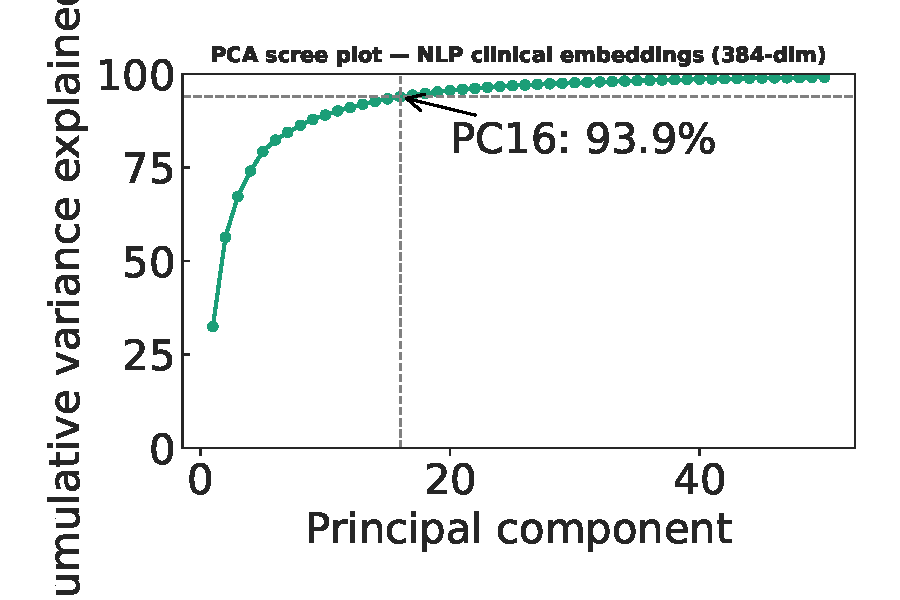
\includegraphics[width=0.7\textwidth]{figures/figS1_pca_scree.pdf}
  \caption{PCA scree plot for the 384-dimensional NLP sentence embeddings.
    The x-axis shows the principal component number (1--50) and the y-axis
    shows cumulative variance explained (\%). The first 16 components
    (vertical dashed line, used as ``NLP-PCA16'') jointly explain
    $\approx$94\% of total variance.}
  \label{fig:supp_pca_scree}
\end{figure}

\begin{figure}[H]
  \centering
  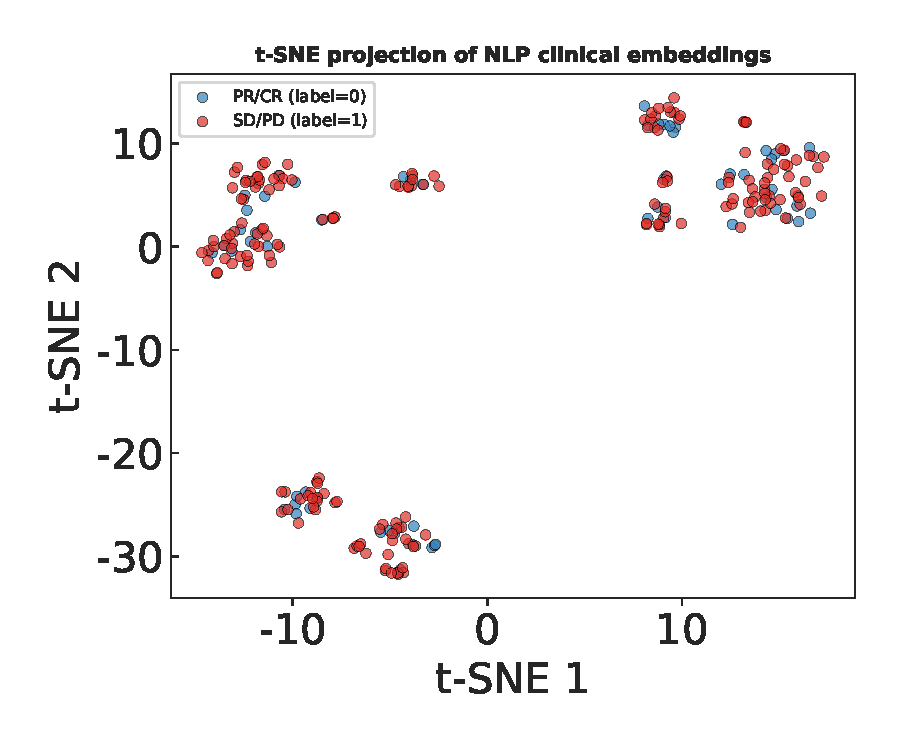
\includegraphics[width=0.7\textwidth]{figures/figS2_tsne_embeddings.pdf}
  \caption{Two-dimensional t-SNE projection of the 384-dimensional NLP
    clinical embeddings for all $n = 247$ discovery-cohort patients,
    coloured by binary outcome (blue: PR/CR, label~$=0$; red: SD/PD,
    label~$=1$). The substantial overlap between classes is consistent with
    the embeddings encoding general clinical/prognostic similarity rather
    than a strong linear separation of binary treatment response.}
  \label{fig:supp_tsne}
\end{figure}

\begin{figure}[H]
  \centering
  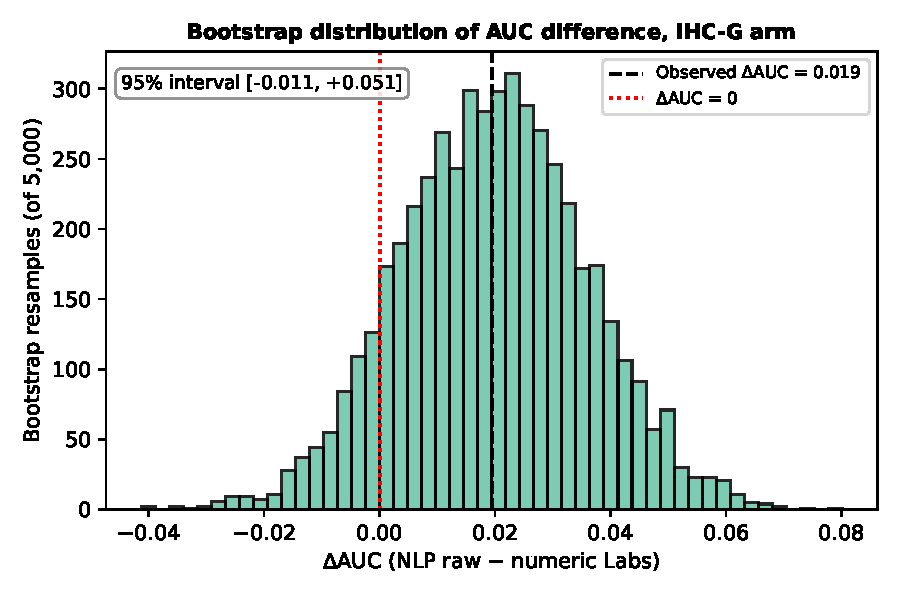
\includegraphics[width=0.7\textwidth]{figures/figS3_bootstrap_pvalue.pdf}
  \caption{Bootstrap distribution of $\Delta\text{AUC}$ (NLP raw $-$ numeric
    Labs, IHC-G arm) across 5{,}000 paired patient-level bootstrap resamples of the
    discovery cohort, using the out-of-fold risk scores of the single 10-fold partition.
    The vertical dashed line marks the observed $\Delta\text{AUC} = 0.019$; the 95\% bootstrap
    interval is $[-0.012, +0.051]$.}
  \label{fig:supp_bootstrap}
\end{figure}

\begin{figure}[H]
  \centering
  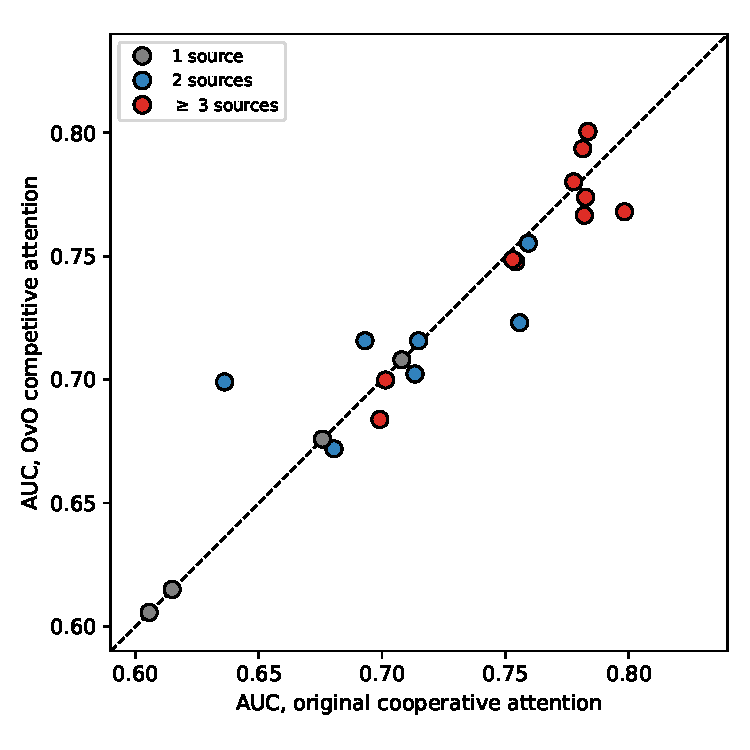
\includegraphics[width=0.7\textwidth]{figures/figS4_ovo_scatter.pdf}
  \caption{Scatter plot comparing AUC under the original cooperative
    attention (x-axis) versus OvO competitive attention (y-axis) across all
    21 tested modality configurations (single 10-fold partition, natural patient order). The diagonal line indicates equal
    performance. Points are coloured by the number of fused modalities
    (grey: 1 modality, where OvO reduces to the original formulation; blue:
    2 modalities; red: $\geq$3 modalities). Points above the diagonal
    indicate configurations where OvO attention improved AUC.}
  \label{fig:supp_ovo_scatter}
\end{figure}

\begin{figure}[H]
  \centering
  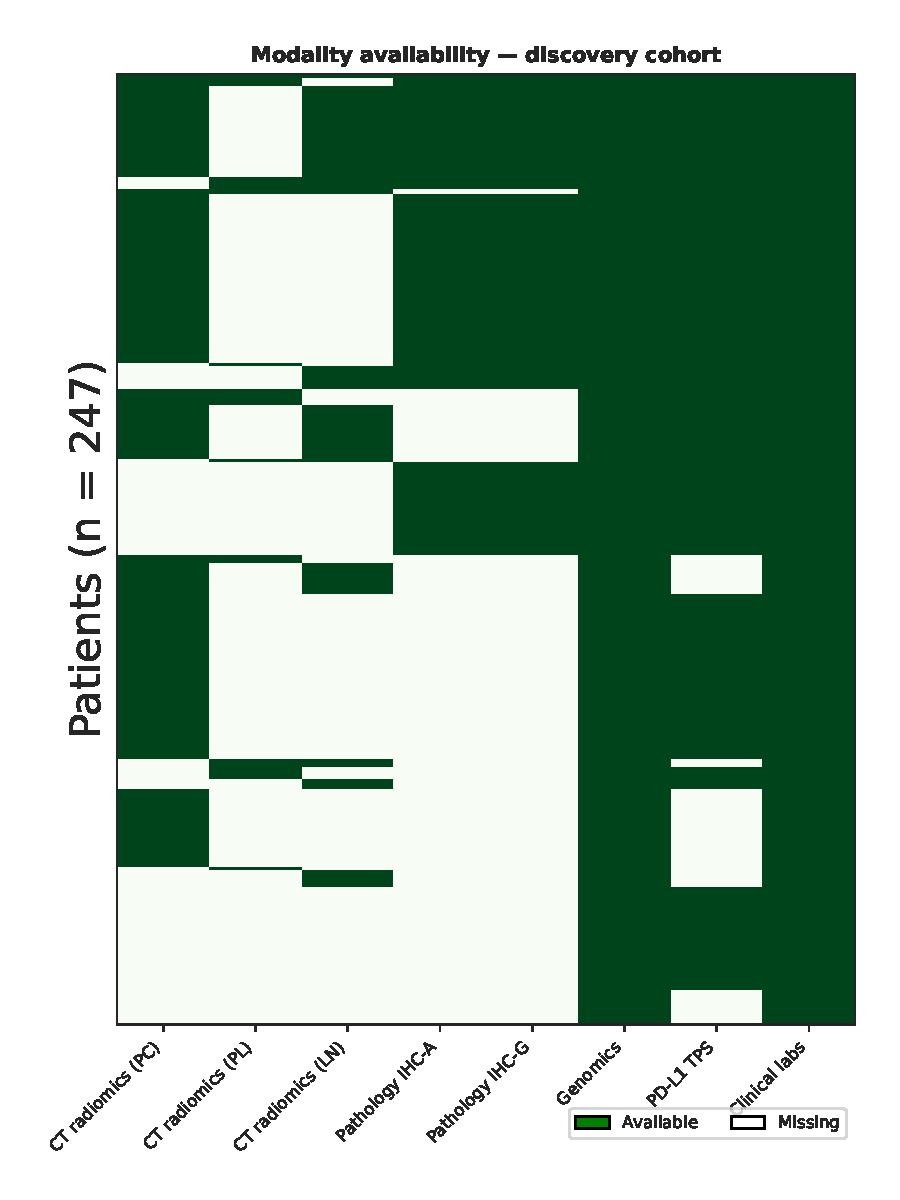
\includegraphics[width=0.7\textwidth]{figures/figS5_modality_heatmap.pdf}
  \caption{Modality availability heatmap for the discovery cohort
    ($n = 247$ patients $\times$ 8 modalities/sub-modalities: CT radiomics
    PC/PL/LN, pathology IHC-A, pathology IHC-G, genomics, PD-L1~TPS, and
    clinical labs). Green indicates the modality is available for a given
    patient; white indicates missing data, handled via the binary
    missingness mask described in the Methods section of the main text.}
  \label{fig:supp_heatmap}
\end{figure}

\section{Supplementary Tables}

\begin{table}[H]
\centering
\caption{Modality availability in the discovery cohort ($n = 247$).
  Counts are taken from the binary missingness mask actually used by the
  fusion model (\texttt{modality\_MASK}), so they are the number of patients
  contributing that modality during training. A patient may contribute
  lesions at more than one anatomical site; the ``any site'' row is the
  union used for the CT radiomics entry of Table~1 of the main text.}
\label{tab:supp_modality}
\begin{tabular}{lcc}
\toprule
\textbf{Modality} & \textbf{Patients available} & \textbf{Coverage (\%)} \\
\midrule
CT radiomics (PC lesion)   & 163 & 66.0  \\
CT radiomics (PL lesion)   & 21  & 8.5   \\
CT radiomics (LN lesion)   & 67  & 27.1  \\
CT radiomics (any site)    & 187 & 75.7  \\
Pathology IHC-A            & 105 & 42.5  \\
Pathology IHC-G (GLCM)     & 105 & 42.5  \\
Genomics (MSK-IMPACT) & 247 & 100.0 \\
PD-L1~TPS                  & 201 & 81.4  \\
Clinical labs (13 variables) & 247 & 100.0 \\
\bottomrule
\end{tabular}
\end{table}

\begin{table}[H]
\centering
\caption{Feature counts per modality before and after feature selection.
  Only the CT radiomics modalities pass through the ICC-based robustness
  filter (ICC~$>0.15$), outlier filter (z-score~$<6$) and elastic-net L1
  selection described in the Methods section of the main text; all other
  modalities enter the model at full dimensionality.
  Because the selection is refitted inside every training fold (the held-out
  fold is excluded before fitting, to avoid selection leakage), the number
  of retained radiomics features varies by fold and is reported as the
  median across the 10 folds with the observed range in brackets.}
\label{tab:supp_features}
\begin{tabular}{lccc}
\toprule
\textbf{Modality} & \textbf{Raw features} & \textbf{After selection} &
\textbf{Retention (\%)} \\
\midrule
CT radiomics (PC lesion)       & 1688 & 35.5 [24--45] & 2.1 \\
CT radiomics (PL lesion)       & 1688 & 7.5 [1--13]  & 0.4 \\
CT radiomics (LN lesion)       & 1688 & 25 [21--41] & 1.5 \\
Pathology IHC-A                & 18   & 18           & 100.0 \\
Pathology IHC-G (GLCM)         & 150  & 150          & 100.0 \\
Genomics                       & 11   & 11           & 100.0 \\
PD-L1~TPS                      & 1    & 1            & 100.0 \\
Clinical labs                  & 13   & 13           & 100.0 \\
NLP raw (MiniLM-L6-v2)         & 384  & 384 (no\_scale) & 100.0 \\
NLP-PCA16                      & 16   & 16 (no\_scale)  & 100.0 \\
\bottomrule
\end{tabular}
\end{table}


\bibliographystyle{plain}
\bibliography{../references}

\clearpage
\section{Survival Analysis by Clinical Encoding}

The clinical-encoding variants of the IHC-A and IHC-G arms (DyAM, single 10-fold partition) and the time-dependent AUC of the 21 configurations.

%% tables/table_s_tdauc21.tex  (GENERATED by make_surv21_tables.py - do not edit by hand)
\begin{table}[H]
\centering
\caption{Time-dependent AUC (Uno estimator) at 6 / 12 / 18 months for the 21 configurations, single 10-fold partition. The +NLP entries are shown only for configurations 20 and 21, where NLP replaces the numeric labs (the other configurations contain no clinical source).}
\label{tab:supp_tdauc21}
\scriptsize
\setlength{\tabcolsep}{3pt}
\begin{tabular}{@{}rlcccc@{}}
\toprule
\# & Configuration & DyAM & OvO & DyAM+NLP & OvO+NLP \\
\midrule
1  & TMB                            & 0.607 / 0.596 / 0.603 & 0.607 / 0.596 / 0.603 & --- & --- \\
2  & PDL1                           & 0.630 / 0.662 / 0.654 & 0.630 / 0.662 / 0.654 & --- & --- \\
3  & IHC-A                          & 0.579 / 0.577 / 0.509 & 0.579 / 0.577 / 0.509 & --- & --- \\
4  & Gen                            & 0.653 / 0.661 / 0.603 & 0.653 / 0.661 / 0.603 & --- & --- \\
5  & Rad                            & 0.612 / 0.651 / 0.681 & 0.600 / 0.646 / 0.664 & --- & --- \\
6  & Rad-LU                         & 0.610 / 0.612 / 0.604 & 0.615 / 0.603 / 0.613 & --- & --- \\
7  & TMB+PDL1                       & 0.592 / 0.589 / 0.519 & 0.646 / 0.617 / 0.567 & --- & --- \\
8  & PDL1+Gen (BM4)                 & 0.649 / 0.630 / 0.596 & 0.668 / 0.654 / 0.625 & --- & --- \\
9  & Rad+IHC-A                      & 0.612 / 0.613 / 0.581 & 0.623 / 0.642 / 0.641 & --- & --- \\
10 & Rad+IHC-G                      & 0.628 / 0.636 / 0.638 & 0.623 / 0.623 / 0.630 & --- & --- \\
11 & Rad+Gen (BM3)                  & 0.692 / 0.715 / 0.713 & 0.706 / 0.730 / 0.715 & --- & --- \\
12 & IHC-A+Gen                      & 0.675 / 0.654 / 0.597 & 0.687 / 0.658 / 0.597 & --- & --- \\
13 & IHC-G+Gen                      & 0.702 / 0.644 / 0.572 & 0.689 / 0.618 / 0.549 & --- & --- \\
14 & Rad+IHC-A+Gen                  & 0.703 / 0.695 / 0.679 & 0.707 / 0.718 / 0.646 & --- & --- \\
15 & Rad+IHC-G+Gen                  & 0.713 / 0.698 / 0.669 & 0.712 / 0.705 / 0.638 & --- & --- \\
16 & Rad+IHC-A+MutAmp               & 0.688 / 0.710 / 0.683 & 0.658 / 0.694 / 0.647 & --- & --- \\
17 & Rad+IHC-A+Gen+PDL1             & 0.767 / 0.774 / 0.760 & 0.711 / 0.732 / 0.669 & --- & --- \\
18 & Rad+IHC-G+Gen+PDL1 (BM1)       & 0.736 / 0.726 / 0.673 & 0.734 / 0.717 / 0.660 & --- & --- \\
19 & Rad+IHC-A+Gen+TMB+PDL1         & 0.700 / 0.712 / 0.647 & 0.708 / 0.725 / 0.670 & --- & --- \\
20 & Rad+IHC-A+Gen+PDL1+Labs        & 0.700 / 0.690 / 0.640 & 0.696 / 0.698 / 0.641 & 0.699 / 0.693 / 0.641 & 0.706 / 0.731 / 0.674 \\
21 & Rad+IHC-G+Gen+PDL1+Labs (BM2)  & 0.719 / 0.698 / 0.643 & 0.721 / 0.709 / 0.664 & 0.715 / 0.702 / 0.650 & 0.730 / 0.733 / 0.690 \\
\bottomrule
\end{tabular}
\end{table}

%% tables/table4_survival.tex  (GENERATED by make_tables_single.py - do not edit by hand)
\begin{table}[H]
\caption{Survival analysis across model variants, from a single 10-fold partition of the fused risk score.
  Discovery cohort ($n = 247$; 209 events, 84.6\%; median PFS 2.7~months). C-index: Harrell's concordance
  index. Cox HR: hazard ratio per unit of risk score from multivariate Cox regression adjusted for age,
  ECOG, albumin, dNLR, and liver metastases. tdAUC: cumulative/dynamic time-dependent AUC at 6, 12 and
  18 months (Uno estimator).}
\label{tab:supp_survival}
\small
\footnotesize
\begin{tabular}{@{}p{3.9cm}ccccc@{}}
\toprule
\textbf{Model} & \textbf{C-index} & \textbf{Cox HR} & \textbf{tdAUC 6~mo} & \textbf{12~mo} & \textbf{18~mo} \\
\midrule
\multicolumn{6}{l}{\textit{IHC-A arm}} \\
No clinical (baseline)         & 0.625 & 5.76 & 0.718 & 0.723 & 0.719 \\
+ Labs (13-dim numeric)        & 0.631 & 5.23 & 0.710 & 0.702 & 0.649 \\
+ NLP raw (384-dim)            & 0.623 & 5.81 & 0.700 & 0.708 & 0.649 \\
+ NLP-PCA16 (16-dim)           & 0.628 & 5.97 & 0.711 & 0.715 & 0.658 \\
+ Labs + NLP (combined)        & 0.616 & 5.23 & 0.696 & 0.705 & 0.673 \\
+ Labs + NLP-PCA16 (combined)  & 0.621 & 5.40 & 0.706 & 0.715 & 0.680 \\
+ BioClinBERT-PCA16            & 0.630 & 6.28 & 0.713 & 0.722 & 0.663 \\
\midrule
\multicolumn{6}{l}{\textit{IHC-G arm}} \\
No clinical (baseline)         & 0.633 & 4.96 & 0.720 & 0.702 & 0.689 \\
+ Labs (13-dim numeric)        & 0.644 & 5.55 & 0.727 & 0.700 & 0.661 \\
+ NLP raw (384-dim)            & 0.627 & 5.64 & 0.713 & 0.700 & 0.653 \\
+ NLP-PCA16 (16-dim)           & 0.629 & 5.57 & 0.715 & 0.697 & 0.647 \\
\bottomrule
\end{tabular}
\end{table}

%% tables/table5_km.tex  (GENERATED by make_tables_single.py - do not edit by hand)
\begin{table}[H]
\caption{Kaplan--Meier log-rank statistics for survival stratification from a single 10-fold partition.
  Patients were dichotomised at the median risk score; $\chi^2 > 3.84$ corresponds to $p < 0.05$ and
  $\chi^2 > 7.88$ to $p < 0.005$ (1 d.f.).}
\label{tab:supp_km}
\begin{tabular}{llc}
\toprule
\textbf{Model} & \textbf{IHC arm} & \boldmath{$\chi^2$} \\
\midrule
No clinical (baseline)         & IHC-A & 23.2 \\
+ Labs (13-dim numeric)        & IHC-A & 18.0 \\
+ NLP raw (384-dim)            & IHC-A & 21.8 \\
+ NLP-PCA16 (16-dim)           & IHC-A & 27.7 \\
+ Labs + NLP (combined)        & IHC-A & 19.9 \\
+ Labs + NLP-PCA16 (combined)  & IHC-A & 22.3 \\
+ BioClinBERT-PCA16            & IHC-A & 20.3 \\
No clinical (baseline)         & IHC-G & 17.8 \\
+ Labs (13-dim numeric)        & IHC-G & 17.9 \\
+ NLP raw (384-dim)            & IHC-G & 18.9 \\
+ NLP-PCA16 (16-dim)           & IHC-G & 20.9 \\
\bottomrule
\end{tabular}
\end{table}


\begin{figure}[H]
  \centering
  \subfloat[IHC-A, no clinical]{%
    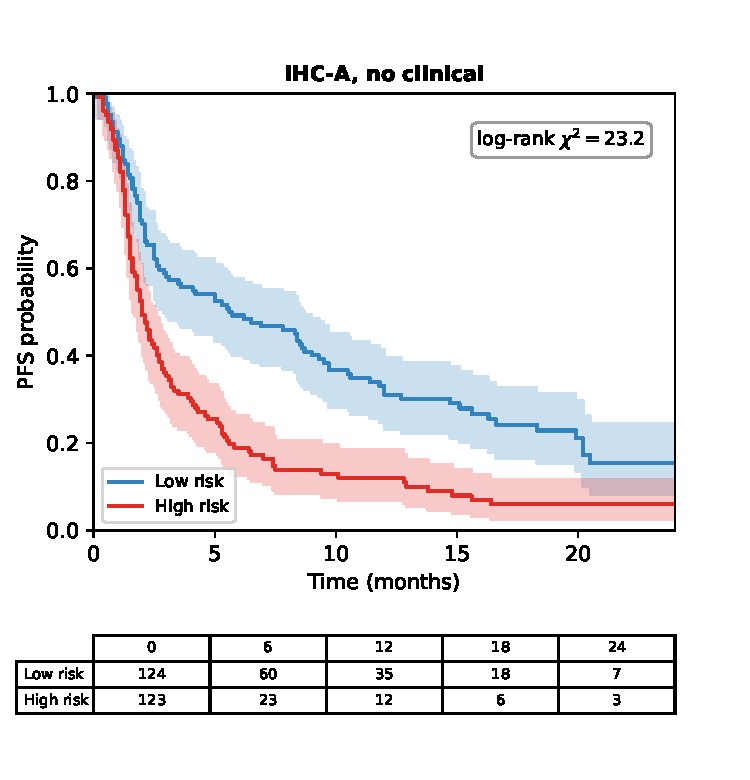
\includegraphics[width=0.48\textwidth]{figures/figS6a_km_ihca_noclin.pdf}}
  \hfill
  \subfloat[IHC-A, + NLP-PCA16]{%
    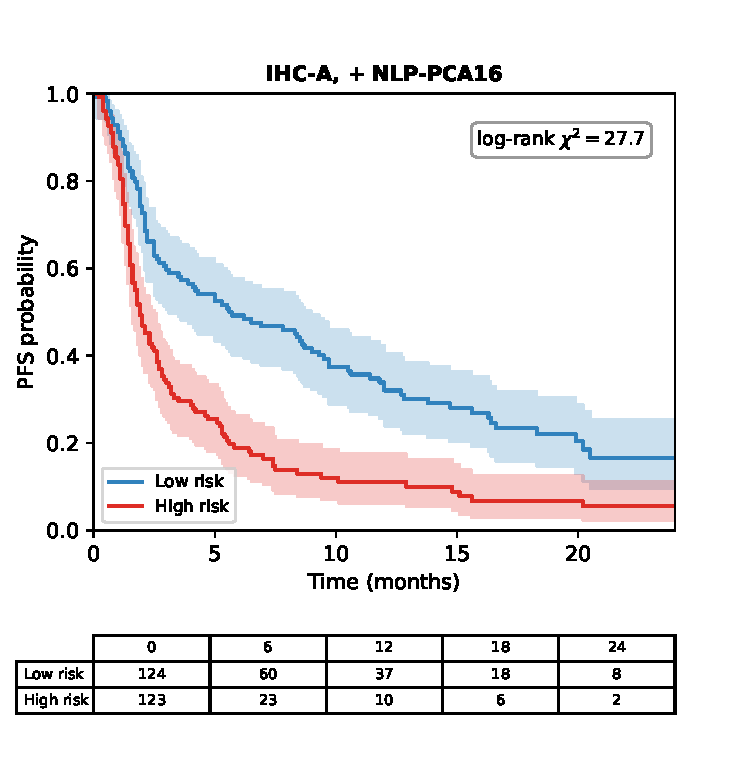
\includegraphics[width=0.48\textwidth]{figures/figS6b_km_ihca_nlppca16.pdf}}

  \subfloat[IHC-G, no clinical]{%
    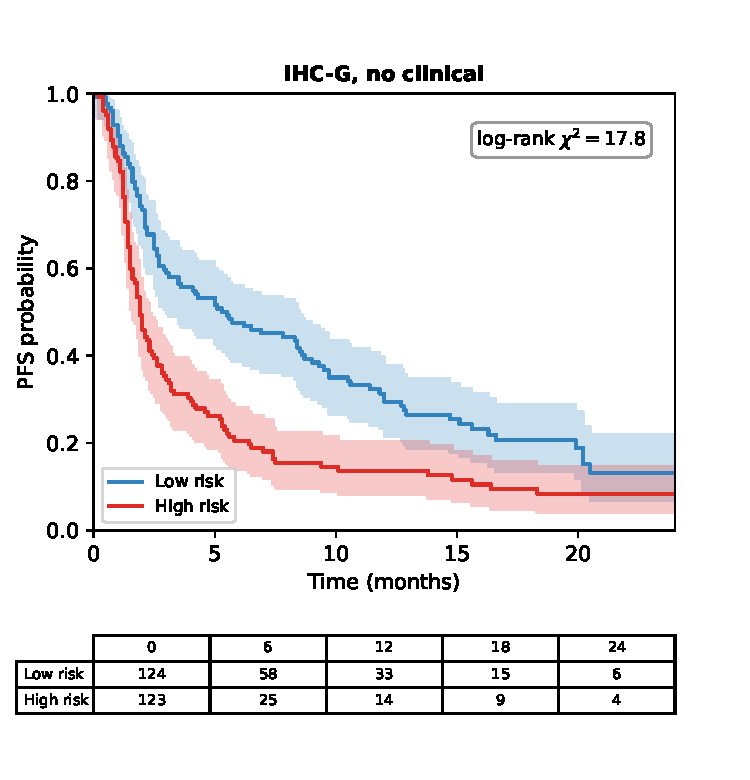
\includegraphics[width=0.48\textwidth]{figures/figS6c_km_ihcg_noclin.pdf}}
  \hfill
  \subfloat[IHC-G, + NLP raw]{%
    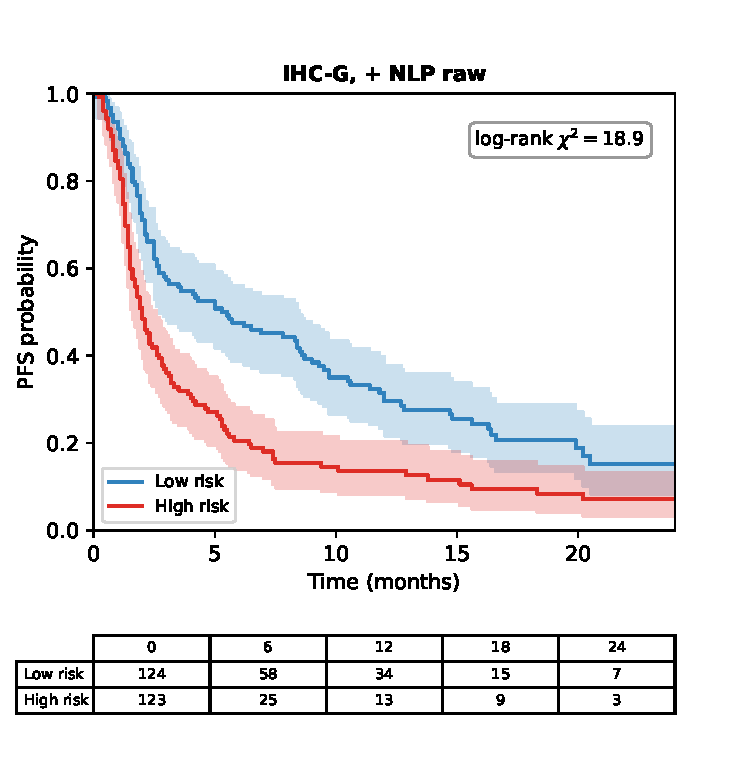
\includegraphics[width=0.48\textwidth]{figures/figS6d_km_ihcg_nlpraw.pdf}}

  \caption{Kaplan--Meier curves for four clinical-encoding variants (single partition; log-rank statistics as in Supplementary Table \ref{tab:supp_km}).}
\end{figure}

\begin{figure}[H]
  \centering
  \subfloat[C-index]{%
    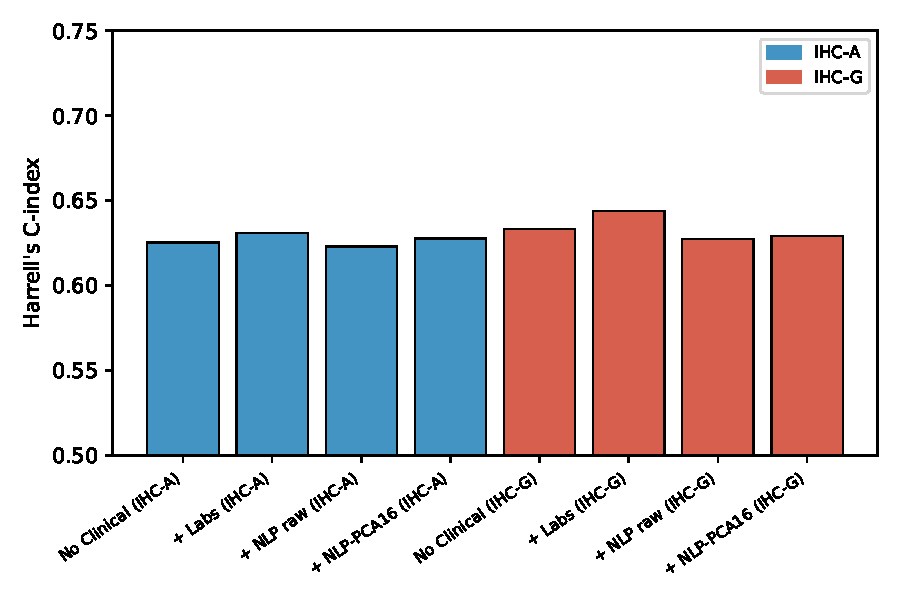
\includegraphics[width=0.48\textwidth]{figures/figS7a_cindex.pdf}}
  \hfill
  \subfloat[Time-dependent AUC]{%
    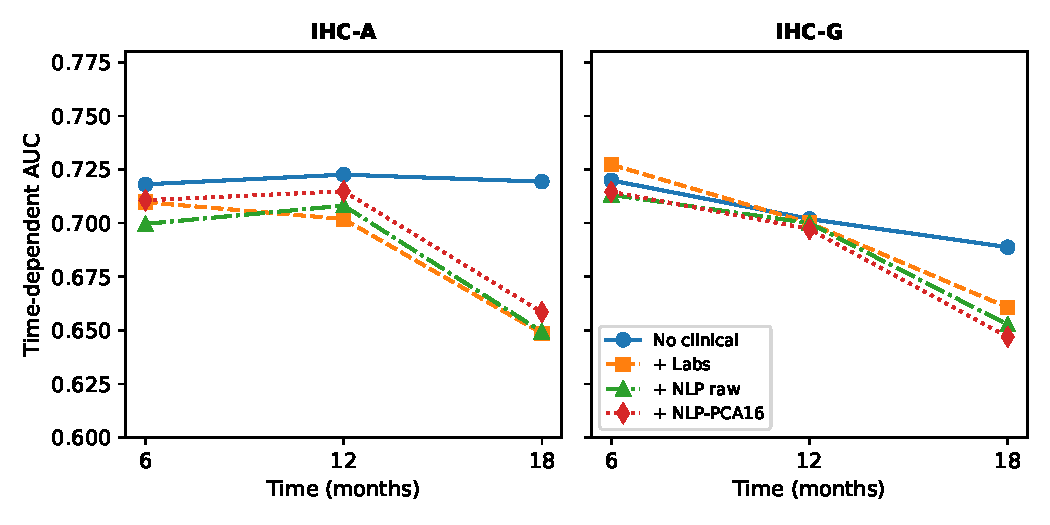
\includegraphics[width=0.48\textwidth]{figures/figS7b_tdauc.pdf}}

  \subfloat[Cox hazard ratio]{%
    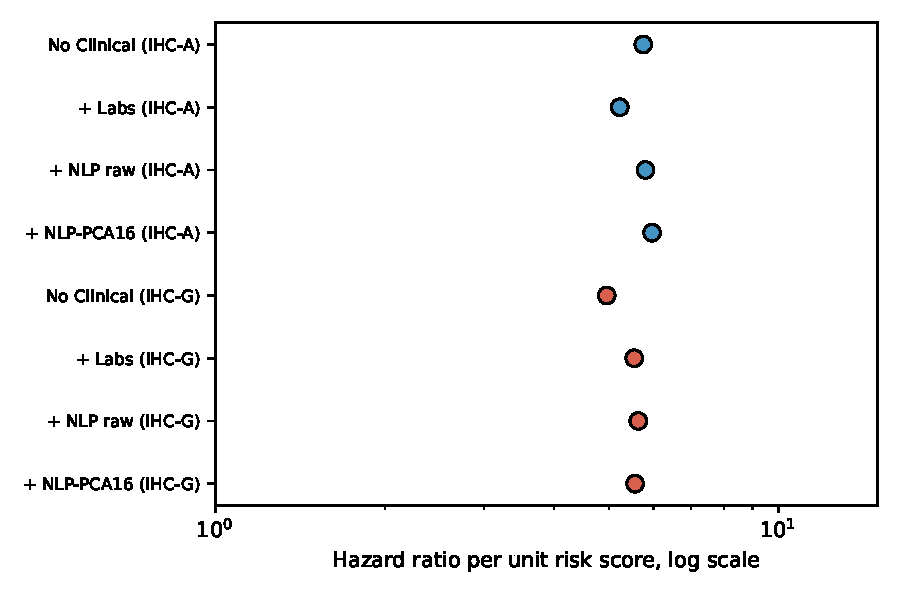
\includegraphics[width=0.48\textwidth]{figures/figS7c_cox_forest.pdf}}
  \hfill
  \subfloat[Log-rank $\chi^2$]{%
    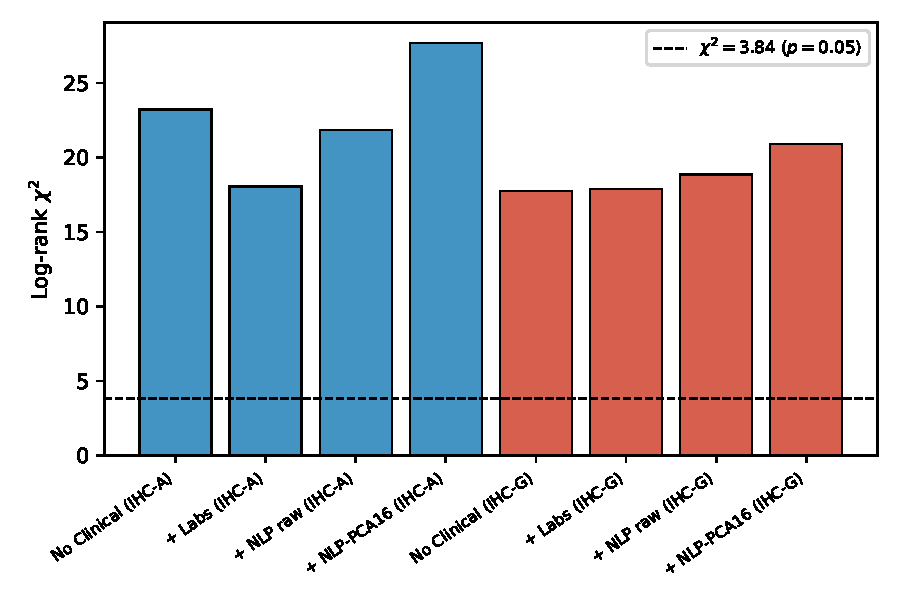
\includegraphics[width=0.48\textwidth]{figures/figS7d_km_chi2.pdf}}

  \caption{Survival metrics across clinical-encoding variants in the IHC-A and IHC-G arms (single partition).}
\end{figure}

\end{document}
